\documentclass[a4paper]{article}
\usepackage[pdftex]{graphicx}
\usepackage[utf8]{inputenc}
\usepackage{enumerate}
\usepackage{siunitx}
\sisetup{locale=DE} 
\usepackage{icomma}
\usepackage{amssymb}
\usepackage{tikz}
\usepackage{href-ul}
\hypersetup{
	colorlinks=true,
	linkcolor=blue,
	urlcolor=blue}
\usepackage{geometry}
\geometry{a4paper, top=15mm, left=15mm, right=15mm, bottom=15mm,
	headsep=10mm, footskip=12mm}

\begin{document}
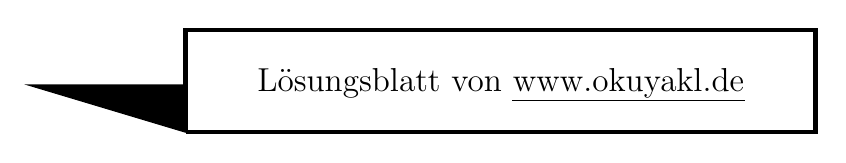
\begin{tikzpicture}(10,3)
	\draw[ultra thick](2,0) --(10,0) -- (10,1.3) --(2,1.3) -- (2,0);
	\draw[fill=black](2,0)-- (0,.6) -- (2,.6) -- (2,0);
	\node at (6,.6) {\large Lösungsblatt von \href{https://www.okuyakl.de}{www.okuyakl.de}};
\end{tikzpicture}
\vspace{0.5 cm}

\noindent{\bf Aufgabe 1.}\\
\begin{itemize}
	\item {\bf Wärmeleitung} findet an der Stelle statt, wo sich zwei Körper unterschiedlicher Temperatur berühren.  
	\item {\bf Wärmestrahlung :} Die Oberfläche eines warmen Körpers gibt Infrarotstrahlung ab.
	\item {\bf Konvektion:} Erwärmte Flüssigkeit oder erwärmtes Gas steigt auf und transportiert Wärme nach oben.
\end{itemize}

\noindent{\bf Aufgabe 2. a)}\\
Die Temperaturkurve dieses Stoffs besitzt Haltepunkte bei $\SI{0}{\celsius}$ und $\SI{100}{\celsius}$, also handelt es sich um Wasser.

\noindent{\bf Aufgabe 2. b)}\\ 
Alle Begriffe beschreiben Phasenübergänge, Tabelle ist zeilenweise zu lesen. 

\renewcommand{\arraystretch}{2}
\begin{tabular}{|c|c|c|c|}
\hline
Phase & fest & flüssig & gasförmig \\
\hline
fest  &  -  &  schmelzen & sublimieren \\
\hline 
flüssig & erstarren & - & sieden \\
\hline 
gasförmig & resublimieren & kondensieren & - \\
\hline 
\end{tabular} 
\vspace{0.5 cm}

\noindent{\bf Aufgabe 2. c)}\\
\begin{itemize}
	\item {\bf Punkt A:} Feste Phase: Eis wird erwärmt bis zum Schmelzpunkt 
	\item {\bf Punkt B:} Schmelzvorgang: Während des Schmelzens verharrt die Temperatur solange bei $273~K$, bis kein Eis mehr da ist.
	\item {\bf Punkt C:} Flüssige Phase: Wasser erwärmt sich kontinuierlich bis zum Siedepunkt.
	\item {\bf Punkt D:} Das Wasser kocht
	\item {\bf Punkt E:} Alles Wasser ist verdampft, der Dampf erwärmt sich nun weiter.
\end{itemize} 
\vspace{0.5 cm}

\noindent{\bf Aufgabe 3. a)}\\
Zum Schmelzen des Eises benötigen wir die Wärmemenge:
$$Q_s = s_{H_2O}\cdot m = \SI{334}{\kilo\joule\over \kilogram} \cdot \SI{0,16}{\kilogram} = \SI{53,4}{\kilo\joule}$$
Zum Erwärmen des nun flüssigen Wassers wird benötigt:
$$Q_c = c_{H_2O}\cdot m \cdot \Delta \vartheta = \SI{4,18}{\kilo\joule\over \kilogram\kelvin}\cdot \SI{0,16}{\kilogram} \cdot \SI{100}{\kelvin}= \SI{66,9}{\kilo\joule}$$
Das Verdampfen des Wassers erfordert die Wärmemenge:
$$Q_r = r_{H_2O}\cdot m = \SI{2257}{\kilo\joule\over \kilogram}\cdot \SI{0,16}{\kilogram} = \SI{361}{\kilo\joule}$$
Zum Verdampfen des Eises ist also die Wärmemenge nötig:
$$Q_{ges}=Q_s + Q_c + Q_r  = \SI{481}{\kilo\joule}$$
\vspace{0.5 cm}

\noindent{\bf Aufgabe 3. b)}\\
Hier ist die Leistung gleich Wärmemenge pro Zeit und wir formen um:
$$ P = {Q \over t} \quad \Rightarrow \quad t = {Q \over P} = {\SI{481e3}{\joule}\over \SI{2800}{\watt}}=\SI{172}{\second} $$
Die Heizdauer beträgt somit rund drei Minuten. 
\vspace{0.5 cm}

\noindent{\bf Aufgabe 4. a)}\\ 
Ein Bimetallstreifen besteht aus zwei Schichten unterschiedlicher Metalle, die sich bei Wärme ebenfalls unterschiedlich ausdehnen. Dadurch biegt sich der Streifen bei Erwärmung in Richtung des Metalls mit der kleineren Wärmeausdehnung, bei Abkühlung in die andere Richtung.
\vspace{0.5 cm}

\noindent{\bf Aufgabe 4. b)}\\
Dies ist ein Thermostat, ein üblicherweise bei Heizvorrichtungen eingebauter Schalter, der diese bei Unterschreiten einer bestimmten Temperatur einschaltet und sie bei Überschreiten einer bestimmten Temperatur ausschaltet.
\vspace{0.5 cm}

\noindent{\bf Aufgabe 5.}\\
Die Zimmertemperatur von $\SI{19}{\celsius}$ in Kelvin ist:
$$T_K = T_C + 273,15 = 19 + 273,15 = \SI{292,15}{\kelvin} K$$ 
Der Siedepunkt von Sauerstoff liegt bei $\SI{90}{\kelvin}$, also muss die Luft um
$$\SI{292,15}{\kelvin}- \SI{90}{\kelvin} \approx \SI{202}{\kelvin}$$ 
abgekühlt werden, um ihn zu verflüssigen.
\vspace{0.5 cm}

\noindent{\bf Aufgabe 6. a)}\\
Die von der Wassermenge $m_2$ aufgenommene Wärmemenge ist nach der Kondensation:
$$Q_2=c_{H_2O}\cdot m_2 \cdot (82-20)\SI{}{\kelvin} = \SI{4,2}{\kilo\joule\over \kilogram\kelvin}\cdot \SI{1,8}{\kilogram} \cdot \SI{62}{\kelvin} = 468~kJ$$
\vspace{0.5 cm}

\noindent{\bf Aufgabe 6. b)}\\
Die von dem $\SI{100}{\celsius}$ heißen, kondensierten Wasser der Menge $m_1$ abgegebene Wärmemenge ist:
$$Q_1=c_{H_2O}\cdot m_1 \cdot (100-82)\SI{}{\kelvin} = \SI{4,2}{\kilo\joule\over \kilogram\kelvin}\cdot \SI{0,2}{\kilogram} \cdot \SI{18}{\kelvin} = \SI{15}{\kilo\joule}$$
Die Differenz dieser beiden Werte ist die Wärmemenge, die durch die Kondensation des Wasserdampfes abgegeben wird:
$$Q_k= Q_2-Q_1=\SI{468}{\kilo\joule}-\SI{15}{\kilo\joule}=\SI{453}{\kilo\joule}$$
Nach dem Umstellen der Formel erhalten wir für $r$:
$$Q_k = r\cdot m \quad \Rightarrow \quad r= {Q_k \over m} =\SI{2265}{\kilo\joule\over \kilogram} \approx \SI{2,3e3}{\kilo\joule\over \kilogram} $$
Dieser Wert trifft den oben angegebenen Literaturwert ziemlich gut.
 \vspace{0.5 cm}
 
\noindent{\bf Aufgabe 7.}\\
Das Wasser-Eis-Gemisch hat nun die Temperatur $\SI{0}{\celsius}$. Hier gilt wieder: aufgenommene Wärme = abgegebene Wärme. Die Wassermenge $m_w$ hat die Wärmemenge abgegeben:
$$Q_w = c_{H_2O}\cdot m_w \cdot \Delta \vartheta =\SI{4,2}{\kilo\joule\over \kilogram\kelvin} \cdot \SI{3,2}{\kilogram} \cdot \SI{30}{\kelvin} = \SI{403}{\kilo\joule}$$
Der Massenanteil an geschmolzenem Eis ist:
$$m_{ge}=0,70 \cdot \SI{1,5}{\kilogram}= \SI{1,05}{\kilogram}$$
Zum Schmelzen dieser Eismasse wurde benötigt:
$$Q_s=s_w \cdot m_w = \SI{334}{\kilo\joule\over \kilogram} \cdot \SI{1,05}{\kilogram}=\SI{351}{\kilo\joule}$$
Die Differenz beider Wärmemengen ergibt die vom festen Eis aufgenommene Wärmemenge:
$$Q_e = Q_w-Q_s=\SI{52}{\kilo\joule}$$
Das Eis wurde um folgende Temperatur erwärmt:
$$
\renewcommand{\arraystretch}{2}
\begin{array}{rcll}
Q_e &=& c_{eis}\cdot m_{eis}\cdot \Delta \vartheta &|\: c_{eis} \quad |: m_{eis}\\
\Delta \vartheta &=& {Q_e \over c_{eis}\cdot m_{eis}}\\
\Delta \vartheta &=& {\SI{52}{\kilo\joule}\over \SI{2,1}{\kilo\joule\cdot\kilogram^{-1}\cdot\kelvin^{-1}}\cdot \SI{1,5}{\kilogram}}\\
\Delta \vartheta &=& 17~K
\end{array}
$$ 
Das Eis hatte eine Temperatur von $\SI{-17}{\celsius}$, bevor es ins Wasser gegeben wurde.
\vspace{0.5 cm}

\noindent{\bf Aufgabe 8. a)}\\
Das Metall des Löffels besteht aus einem Atomgitter, in welchem sich benachbarte Atome berühren. Erhitzt man einen Bereich dieses Gitters, so geraten die Atome in stärkere Schwingungen um ihre Ruhelage. Durch Stöße mit benachbarten Atomen erfassen diese Schwingungen schließlich auch weiter entferntere Bereiche des Gitters.
\vspace{0.5 cm}

\noindent{\bf Aufgabe 8. b)}\\
Konvektion findet z.B. in einem Raum mit einem Heizkörper statt. Ein Luftpaket erwärmt sich zunächst durch Kontakt mit der warmen Oberfläche des Heizkörpers. Die erwärmte Luft steigt aufgrund ihrer geringeren Dichte auf und kältere Luft erreicht den Heizkörper, welche wiederum erwärmt wird und aufsteigt. Somit entsteht eine Zirkulation, durch die nach und nach die gesamte Luft des Raums erwärmt wird. 
\vspace{0.5 cm}

\noindent{\bf Aufgabe 9.}\\
Die zugeführte Energie ist gleich der potentiellen. Damit erhalten wir:
$$
\renewcommand{\arraystretch}{2}
\begin{array}{rcll}
m_{ges}\cdot g \cdot h &=& c \cdot m_{br} \cdot \Delta \vartheta & |:c \quad |:m_{br} \\
\Delta \vartheta &=& {m_{ges}\cdot g \cdot h \over  c \cdot m_{br}} \\
\Delta \vartheta &=& {\SI{85}{\kilogram} \cdot \SI{9,81}{\meter\over{\second^2}}\cdot \SI{100}{\meter} \over \SI{480}{\joule\cdot\kilogram^{-1}\cdot\kelvin^{-1}} \cdot \SI{1,0}{\kilogram}} \\
\Delta \vartheta &=& \SI{174}{\kelvin}\\
\end{array}
$$
Die Trommelbremse erwärmt sich um 174~K.
\vspace{0.5 cm}

\noindent{\bf Aufgabe 10.}\\
In einem abgeschlossenen System ist die Summe der Energien konstant:
innere Energie = Wärmemenge + Arbeit
$$E_i = Q + W$$
\vspace{0.5 cm}

\begin{center}
	\includegraphics[width=7 cm]{../../viecher/endcomic.pdf}
	
	Hier geht es zurück zum \href{https://www.okuyakl.de/phys/p9thaL402/aa402.pdf}{Aufgabenblatt}
\end{center}

\end{document}

